\section{System responses}
\subsection{}

\begin{frame}\mccz
\frametitleTC{Foreword}
\framesubtitleTC{}
\myPause
 \begin{columns}
  \column[T]{0.35\textwidth}
   \only<2->{\centering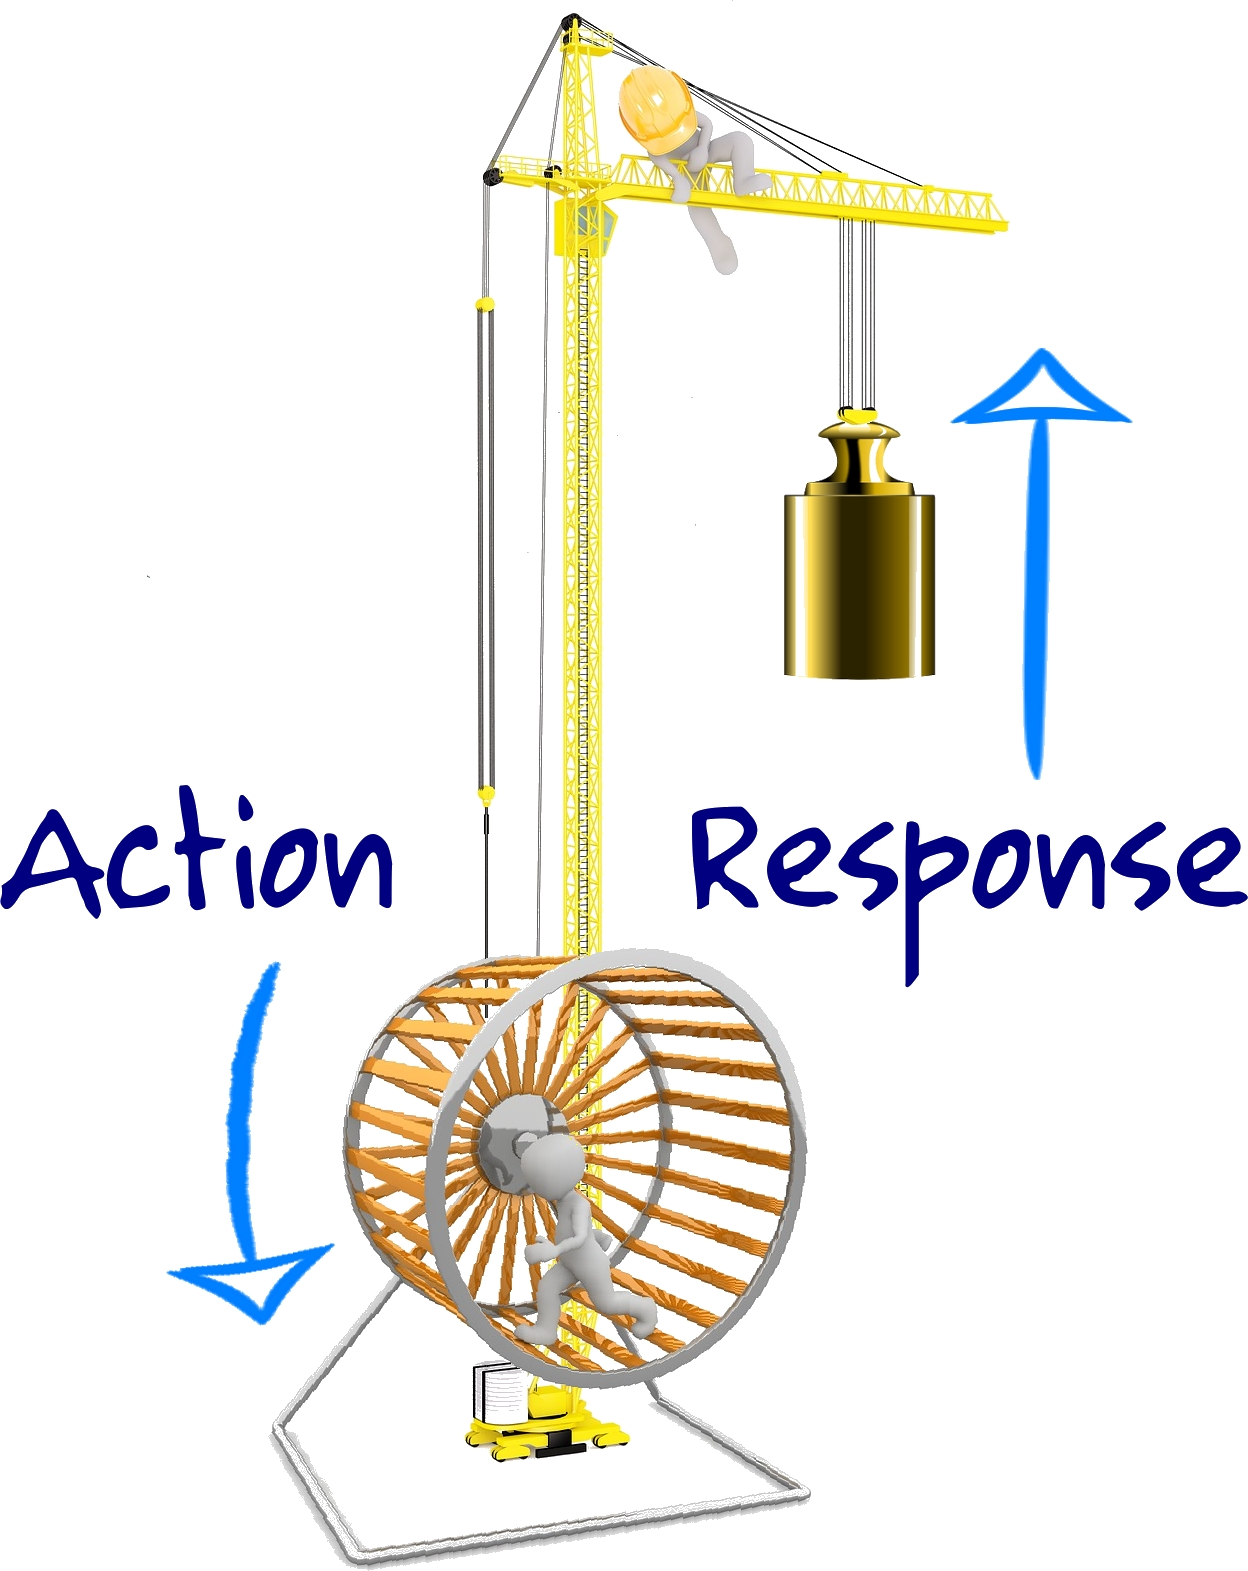
\includegraphics[height=6cm]{./Unit-04/img/response-intro_cc0.jpg}}\myPause%
  \column[T]{0.65\textwidth}
   \begin{itemize}[<+-| alert@+>]
   \item We know how to describe a (DT LTI) dynamic system
         \begin{itemize}[<+-| alert@+>]
         \item in the state space with $(A,b,c,d)$
         \item and with a transfer function $G(z)$.
         \end{itemize}
   \item But how do these descriptions relate to the way\\
         the system responds to a certain \emph{stimulus}?
   \item Specifically for our purpose, can we somehow\\
         relate a transfer function to its\\
         \TC{time (domain) responses}?
   \item \vspace{3mm} Of course we can.
   \item Let us see first how and then why.
   \end{itemize}
 \end{columns}
\end{frame}

\begin{frame}
\frametitleTC{Foreword}
\framesubtitleTC{An introductory case}
\myPause
 \begin{itemize}[<+-| alert@+>]
 \item We showed that as long as a system has only real eigenvalues, its transfer function can be
       expressed as sum/product of elementary first order terms in the form
       \begin{displaymath}
        g(z) = \frac{\mu}{z-p}
       \end{displaymath}
 \item NOTE: if all eigenvalues are distinct, a sum (no products) of terms\\
       like the above suffices.
 \item Given the linearity of the system, responses will sum together the\\
       same way as elementary terms in the transfer function do.
 \item We therefore start by analysing the responses of $g(z)$ above\\
       to a unit impulse and a unit step.
 \item We deal with TI systems, hence in the following everything starts\\
       at $k=0$.
 \end{itemize}
\end{frame}

\begin{frame}
\frametitleTC{An introductory case}
\framesubtitleTC{Impulse response of $g(z)$}
\myPause
 \begin{itemize}[<+-| alert@+>]
 \item Recalling the meaning of $z$, $g(z)$ in the time domain means
       \begin{displaymath}
        y(k) = p y(k-1) + \mu u(k-1).
       \end{displaymath}
 \item Set now $u(k)=imp(k)$, i.e., the sequence $\{1,0,0,0,\ldots\}$. We assume no action on the system
       before $k=0$, consistently with the definition of impulse. We also assume the system at rest, otherwise
       there is free motion and we don not see ONLY the response to $u$, hence $y=0$ for $k<0$.
 \item This said, we get
       {\small
       \begin{displaymath}
        \begin{array}{lclclclclcl}
         y(0) &=& p y(-1) + \mu u(-1) &=& p \cdot 0     + \mu \cdot 0 &=& 0       \\
         y(1) &=& p y(0)  + \mu u(0)  &=& p \cdot 0     + \mu \cdot 1 &=& \mu     \\
         y(2) &=& p y(1)  + \mu u(1)  &=& p \cdot \mu   + \mu \cdot 0 &=& \mu p   \\
         y(3) &=& p y(2)  + \mu u(2)  &=& p \cdot \mu p + \mu \cdot 0 &=& \mu p^2 \\
         \ldots
        \end{array}
       \end{displaymath}
       }
 \item \vspace{-4mm}i.e., the sequence $\{0,\mu,\mu p,\mu p^2,\mu p^3,\ldots\}$.
 \end{itemize}
\end{frame}

\begin{frame}[fragile]
\frametitleTC{An introductory case}
\framesubtitleTC{Impulse response of $g(z)$}
\myPause
 \begin{itemize}[<+-| alert@+>]
 \item Summarising, the impulse response of $g(z)$ is
       \begin{displaymath}
        y(k) = \begin{cases}
                0           & k=0 \\
                \mu p^{k-1} & k>0
               \end{cases}
       \end{displaymath}
 \item Let us compute and plot this response with Scilab:
       {\small
       \begin{verbatim}
 g   = syslin('d',1/(%z-0.5)); // define transfer function ('d' means DT)
 gss = tf2ss(g);               // convert to state space for dsimul
 u   = [1,0,0,0,0,0,0,0,0,0];  // impulse sequence (10 samples)
 y   = dsimul(gss,u);          // compute response
 plot(y,'.');                  // plot (as dots)
       \end{verbatim}
       }
 \item Try different values of $\mu$ and $p$, and comment on the results.
 \end{itemize}
\end{frame}

\begin{frame}
\frametitleTC{An introductory case}
\framesubtitleTC{Impulse response of $g(z)$ -- general remarks}
\myPause
 \begin{itemize}[<+-| alert@+>]
 \item The pole $p$ governs stability as we already know.
 \item For $p=0$ the system is a pure one-step delay.
 \item For $0<p<1$ the response converges monotonically, for $-1<p<0$ oscillating.
 \item In both cases, $p$ governs the convergence speed.
 \item For $p=1$ the response is constant, for $p=-1$ a sustained oscillation\\
       (in both cases for $k>0$, obviously).
 \item Parameter $\mu$ acts as a (signed) scale factor.
 \end{itemize}
\end{frame}

\begin{frame}
\frametitleTC{An introductory case}
\framesubtitleTC{Step response of $g(z)$}
\myPause
 \begin{itemize}[<+-| alert@+>]
 \item Set $u(k)=step(k)$, i.e., the sequence $\{1,1,1,1,\ldots\}$.
 \item We can verify that this yields the response
       \begin{displaymath}
        y(k) = \frac{\mu}{1-p}(1-p^k)
       \end{displaymath}
 \item To this end, we observe that with $\mu=1-p$ we get $y(k) = 1-p^k$:
       {\scriptsize
       \begin{displaymath}
        \begin{array}{lclclclclcl}
         y(0) &=& p \cdot 0       + (1-p) \cdot 0 & &           &=& 0     \\
         y(1) &=& p \cdot 0       + (1-p) \cdot 1 & &           &=& 1-p   \\
         y(2) &=& p \cdot (1-p)   + (1-p) \cdot 1 &=& p-p^2+1-p &=& 1-p^2 \\
         y(3) &=& p \cdot (1-p^2) + (1-p) \cdot 1 &=& p-p^3+1-p &=& 1-p^3 \\
         y(4) &=& p \cdot (1-p^3) + (1-p) \cdot 1 &=& p-p^4+1-p &=& 1-p^4 \\
         y(5) &=& p \cdot (1-p^4) + (1-p) \cdot 1 &=& p-p^5+1-p &=& 1-p^5 \\
         \ldots
        \end{array}
       \end{displaymath}
       }
 \item \vspace{-4mm}Hence a generic $\mu$ scales $y$ to give the result above.
 \end{itemize}
\end{frame}

\begin{frame}[fragile]
\frametitleTC{An introductory case}
\framesubtitleTC{Step response of $g(z)$}
\myPause
 \begin{itemize}[<+-| alert@+>]

 \item Also for the step response case, let us compute and plot some examples with Scilab:
       {\small
       \begin{verbatim}
 g   = syslin('d',1/(%z-0.5)); // define transfer function ('d' means DT)
 gss = tf2ss(g);               // convert to state space for dsimul
 u   = ones(1,10)              // step sequence (a row of 10 samples)
 y   = dsimul(gss,u);          // compute response
 plot(y,'.');                  // plot (as dots)
       \end{verbatim}
       }
 \item Try again different values of $\mu$ and $p$, and comment on the results.
 \end{itemize}
\end{frame}

\begin{frame}
\frametitleTC{An introductory case}
\framesubtitleTC{Step response of $g(z)$ -- general remarks}
\myPause
 \begin{itemize}[<+-| alert@+>]
 \item The pole $p$ governs stability as we already know.
 \item For $p=0$ the system is a pure one-step delay.
 \item For $0<p<1$ the response converges monotonically, for $-1<p<0$ oscillating.
 \item In both cases, $p$ governs the convergence speed.
 \item For $p=1$ the response is a diverging ramp, for $p=-1$ a sustained oscillation.
 \item If $y(k)$ converges, it does so to the value
       \begin{displaymath}
        \frac{\mu}{1-p} = g(1)
       \end{displaymath}
       that is called the \TC{gain} of the transfer function.
 \item Hence for an asymptotically stable $g(z)$, if for $k\rightarrow\infty$ $u(k)\rightarrow\overline{u}$,\\
       then $y(k)\rightarrow g(1)\overline{u}$.
 \end{itemize}
\end{frame}

\begin{frame}
\frametitleTC{Generalisation}
\framesubtitleTC{}
\myPause
 \begin{itemize}[<+-| alert@+>]
 \item In the same way we treated the elementary term $g(z)$, we could address a generic transfer function.
 \item However
       \begin{itemize}[<+-| alert@+>]
       \item as long as there are single poles (eigenvalues), the response will be a linear 
             combination of terms like those yielded by $g(z)$,
       \item while multiple eigenvalues (poles) can be treated like we did from slide~\ref{pag:ex-realisation}
             onward (enough on this for our purposes),
       \item and complex poles could be a nice exercise for the interested \smiley\\
             although here we do not address them either.
       \end{itemize}
 \item We do not treat the most general case, nonetheless we go through\\
       one non-elementary example as this allows for useful considerations.
 \end{itemize}
\end{frame}

\begin{frame}
\frametitleTC{Generalisation}
\framesubtitleTC{One model class, some particular cases}
\myPause
 \begin{itemize}[<+-| alert@+>]
 \item Take the class of transfer functions with up to two poles and one zero
       \begin{displaymath}
        G(z) = \frac{b_0+b_1z}{a_0+a_1z+a_2z^2}
       \end{displaymath}
 \item and specialise it to the four cases
       \begin{displaymath}
        \begin{array}{c}
         G_A(z) = \cfrac{1}{z}, \qquad
         G_B(z) = \cfrac{0.5}{z-0.5}, \qquad
         G_C(z) = \cfrac{(1-0.25)^2}{1-0.55} \, \cfrac{z-0.55}{(z-0.25)^2}, \\ \\
         G_D(z) = \cfrac{2.5-1}{(1-0.5)^2} \, \cfrac{2.5-z}{(z-0.5)^2}.
        \end{array}
       \end{displaymath}
 \item Notice that for clarity in the following plots they all have unity\\
       gain, i.e., $G_{A,B,C,D}(1)=1$.
 \end{itemize}
\end{frame}

\begin{frame}
\frametitleTC{Generalisation}
\framesubtitleTC{One model class, different responses}
\myPause
 \begin{itemize}[<+-| alert@+>]
 \item The corresponding four (unit) step responses are plotted below with the so-called\\
       ``staircase'' style:
       \begin{center}
        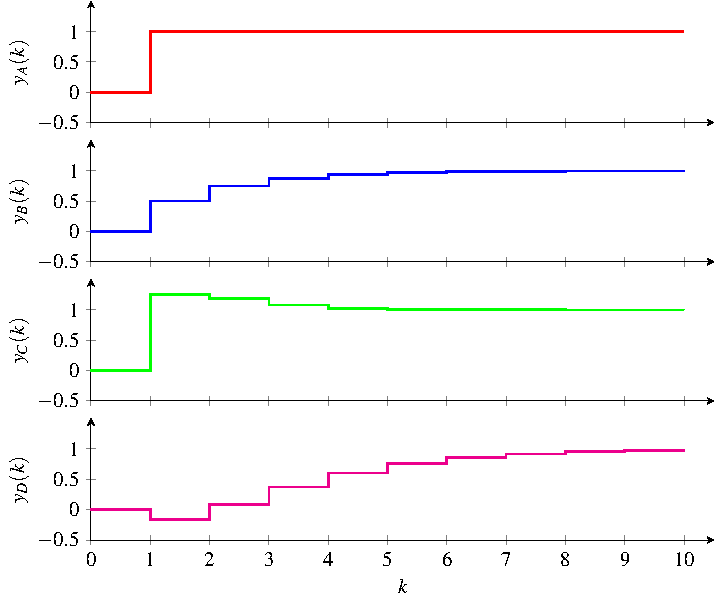
\includegraphics[width=0.50\columnwidth]{./Unit-04/img/StepRespTypes.pdf}
       \end{center}
 \item \vspace{-3mm} Let us try to provide some possible interpretation.
 \end{itemize}
\end{frame}

\begin{frame}
\frametitleTC{Generalisation}
\framesubtitleTC{One model class, different responses}
\myPause
 \begin{columns}
  \column[T]{0.45\textwidth}
   \only<2->{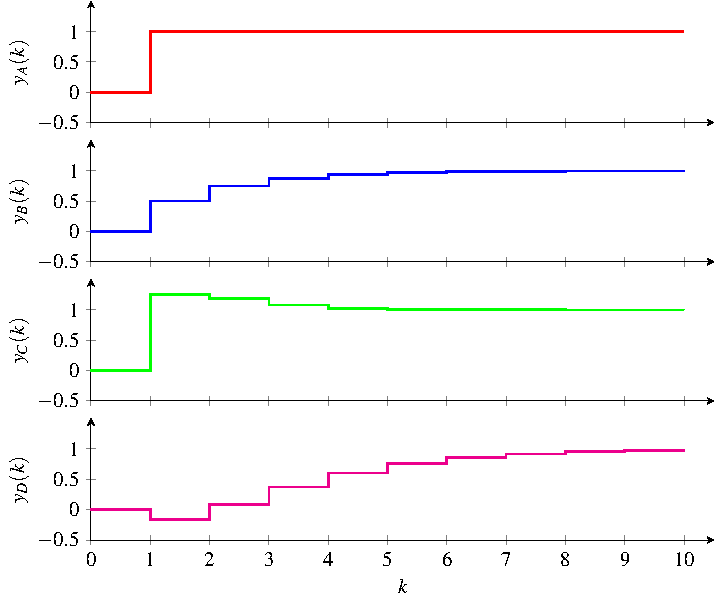
\includegraphics[height=5.5cm]{./Unit-04/img/StepRespTypes.pdf}}
  \column[T]{0.55\textwidth}
   \begin{itemize}[<+-| alert@+>]
   \item Suppose $u(k)$ and $y(k)$ to be respectively a resource to allot and its effect.
         \begin{itemize}[<+-| alert@+>]
         \item[A.] The resource is acquired and exerts immediately its effect (that is therefore
                   seen at the very next step).
         \item[B.] The resource acts immediately but takes some steps to yield its full effect\\
                   (for example because first\\
                   some queue needs\\
                   emptying).
         \end{itemize}
   \end{itemize}
 \end{columns}
\end{frame}

\begin{frame}
\frametitleTC{Generalisation}
\framesubtitleTC{One model class, different responses}
 \begin{columns}
  \column[T]{0.45\textwidth}
   \only<1->{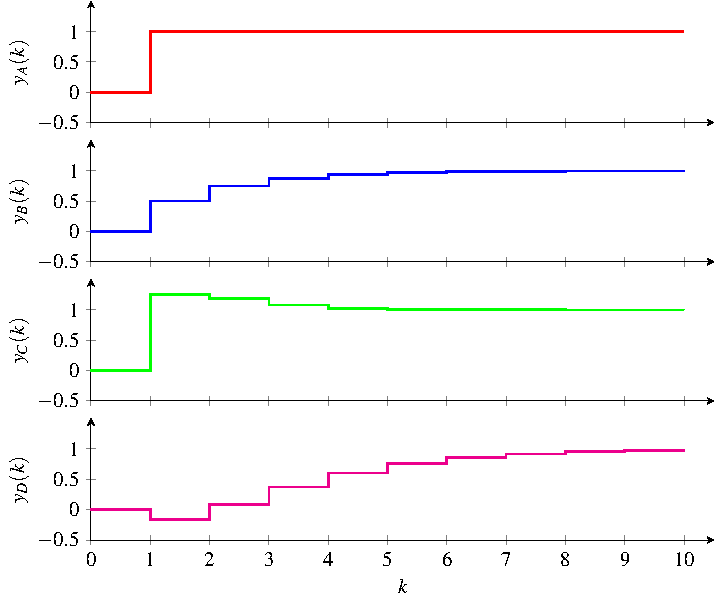
\includegraphics[height=5.5cm]{./Unit-04/img/StepRespTypes.pdf}}
  \column[T]{0.55\textwidth}
   \begin{itemize}[<+-| alert@+>]
   \item Suppose $u(k)$ and $y(k)$ to be respectively a resource to allot and its effect.
         \begin{itemize}[<+-| alert@+>]
         \item[C.] The resource produces a transiently enhanced effect (this is quite typical
                   when the resource is computational power and the effect is the \emph{speed} toward a goal).
         \item[D.] The resource requires some effort to be acquired and initially \emph{reduces}
                   performance, like a new\\
                   core that when acquired\\
                   has an unknown cache\\
                   content, thus causing\\
                   a lot of cache misses.
         \end{itemize}
   \end{itemize}
 \end{columns}
\end{frame}

\begin{frame}
\frametitleTC{Generalisation}
\framesubtitleTC{Lessons learnt and next steps}
\myPause
 \begin{itemize}[<+-| alert@+>]
 \item One model can produce very different responses \TC{by just changing parameters}, thus fitting
       several physical cases --- remember the remark in the introductory section, that we need a systems
       and control theory because determining a controller is largely physics-independent?.
 \item \vspace{3mm} We shall now see how control requirements can be stipulated by saying that some response
       to some \emph{stimulus} should have a certain aspect.
 \item We shall then convert this into requiring some \TC{transfer function}\\
       to have a certain aspect...
 \item ...and finally start synthesising feedback controllers.
 \end{itemize}
\end{frame}

